% This is the Typeset of Merge Sort notes of CS 504
% Author: Prof. Micha Hofri
% Typesetted by Chao Li



\documentclass{article}
\usepackage{pgf}
\usepackage{tikz}
\usetikzlibrary{arrows, automata}
\title{Merge Sort}
\author{Prof. Micha Hofri}
\begin{document}

\maketitle

First, assume we have three numbers $a, b, c$, and we want to 
find the smallest number among them. Let's look at a decision 
tree of the process:\\
\begin{center}
\begin{tikzpicture}[level/.style={sibling distance=60mm/#1}]
  \node (S) {$S$}
    child {node (U1) {$U$}
      child {node (a) {$(a)$}}
      child {node (c1) {$(c)$}}
    }
    child {node (U2) {$U$}
      child {node (c2) {$(c)$}}
      child {node (b) {$(b)$}}
    };
  \path (S)  -- (U1) node [sloped,midway,above] {$a<b$};
  \path (S)  -- (U2) node [midway] {$a>b$};
  \path (U1) -- (a) node [midway] {$a<c$};
  \path (U1) -- (c1) node [midway] {$c<a$};
  \path (U2) -- (c2) node [midway] {$c<b$};
  \path (U2) -- (b) node [midway] {$c>b$};
\end{tikzpicture}
\end{center}
Assume we have two states $U$ and $S$ as above shows, their transition between each
other is shown as follows with the probability of the transition:\\
\begin{center}
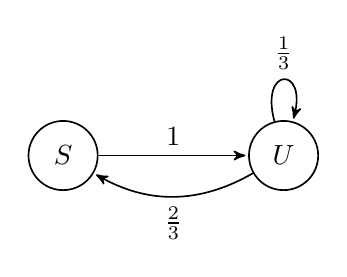
\begin{tikzpicture}[->, >=stealth', shorten >= 1pt, auto, node distance = 2.8cm, semithick]
  \tikzstyle{every state} = [draw, shape = circle]
  \node[state] (S)                 {$S$};
  \node[state] (U) [right of = S]  {$U$};
  \path  (S) edge              node {$1$} (U)
         (U) edge [loop above] node {$\frac{1}{3}$} (U)
         (U) edge [bend left]  node {$\frac{2}{3}$} (S);

\end{tikzpicture}
\end{center}
Then we get:
\begin{center}
$P(S) = P(U) \cdot \frac{2}{3}$\\
$P(U) = P(S) \cdot 1 + P(U) \cdot \frac{1}{3}$
\end{center}
So $P(S) = \frac{2}{5}$, $P(U) = \frac{3}{5}$.\\

Define $c$ as the comparisons per move,\\
Hence $E(c) = 2 \cdot \frac{2}{3} + 1 \cdot \frac{1}{3} =
\frac{5}{3}$\\
Finally, we have\\
\begin{center}
$E(moves\ per\ comparison) = P(U) \cdot 1 = \frac{3}{5}$ \\
$E(comparisons\ per\ move) = \frac{1}{3/5} = \frac{5}{3}$ \\
\end{center}


\end{document}
